\documentclass{nature}

\usepackage{graphicx}
\usepackage{booktabs}
\usepackage{hyperref}
\usepackage{url}
\usepackage{xcolor}

% The local Nature class suppresses \includegraphics because Nature normally
% requests separate figure files. This draft restores embedded figures so the
% exported PDF is presentation-ready.
\let\apcincludegraphics\includegraphics
\AtBeginDocument{\let\includegraphics\apcincludegraphics}
\setlength{\emergencystretch}{3em}
\hypersetup{colorlinks=true,linkcolor=black,citecolor=black,urlcolor=teal}

\title{AutoPlanner-Cascade: process-aware program search for chemoenzymatic synthesis planning}

\author{AutoPlanner-Cascade team$^{1}$}

\begin{document}
\maketitle

\begin{affiliations}
\item AutoPlanner-Cascade project, local research draft generated on 12 May 2026.
\end{affiliations}

\begin{abstract}
Retrosynthesis planners normally search for stock-closed molecule trees. This formulation is useful for route discovery, but it under-specifies cascade synthesis, where feasibility depends on process order, stage boundaries, compatible conditions, cofactors, catalysts and evidence for enzyme modules. We present AutoPlanner-Cascade, a process-aware planning architecture that keeps these constraints inside the search state rather than appending them as post-hoc labels. The current implementation wraps a mature ChemEnzyRetroPlanner multi-step core with coverage-aware access, route-tree tracing, source diagnostics and a learned open-leaf policy. On the local full100 benchmark, coverage-first fixes increased plan rate from 0.76 to 0.97, skeleton type GT@1 from 0.58 to 0.70, candidate exact reaction coverage from 0.24 to 0.40 and candidate GT-reactant coverage from 0.40 to 0.58, while reducing average runtime from 17.68 s to 14.76 s per target. Strict stock closure remains below the previous baseline, identifying stock-aware leaf selection and provider scheduling as the next bottleneck.
\end{abstract}

\section*{Main}
Hybrid organic--enzymatic planning is not only a molecular graph problem. A route that reaches purchasable precursors can still fail as a cascade if adjacent operations require incompatible solvents, pH windows, temperatures, redox states, catalysts or workups. The original ChemEnzyRetroPlanner-style problem is therefore best viewed as a strong route generator, not as a complete process planner.

AutoPlanner-Cascade changes the planning object from a route tree to a partial cascade program. Each search state contains open molecule leaves, reaction history, candidate provenance, stage and condition placeholders, stock status, failure labels and trace features. This makes candidate generation, source scheduling and open-leaf selection measurable during search. Cascade scoring is deliberately introduced as a soft state-level preference, because many useful routes include non-cascade or stock-closing terminal steps.

\begin{center}
\refstepcounter{figure}\label{fig:main}
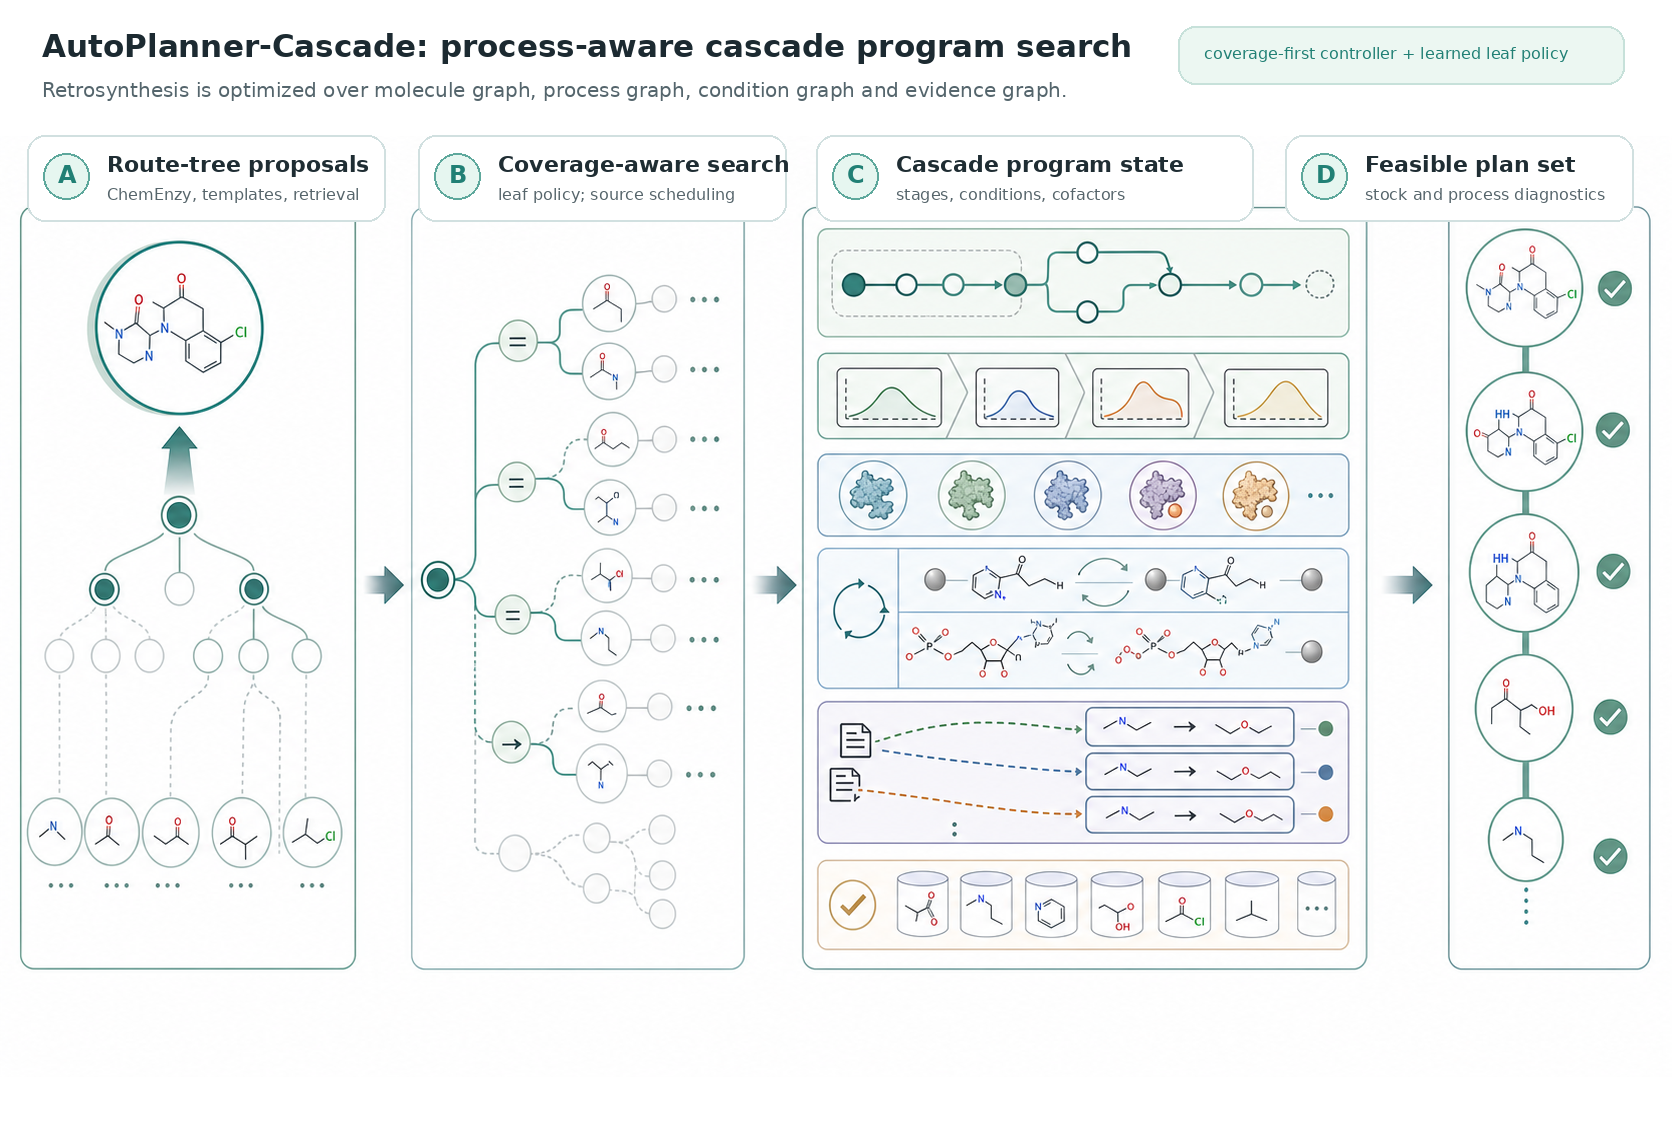
\includegraphics[width=\linewidth]{figures/figure1_cascade_native.png}
\par\small\sffamily\textbf{Figure \thefigure\ $|$ Cascade-native planning as a program search problem.}
\textbf{A,} Mature one-step and multi-step proposal machinery supplies retrosynthetic candidates.
\textbf{B,} A coverage-aware controller records which intermediates are reached, which sources are queried and where candidates are lost.
\textbf{C,} The intended cascade state augments the molecule tree with process stages, condition envelopes, enzyme modules, cofactor ledgers and evidence links.
\textbf{D,} The planner returns ranked program candidates with stock closure and cascade diagnostics, rather than a molecule-only route. The background panel was generated with image2 and labelled deterministically for manuscript use.
\end{center}

\section*{Results}
The first engineering target was not to add another scorer, but to verify that the planner can reach the correct intermediates and expose the right candidate actions. We therefore implemented a coverage audit that separates candidate missing, intermediate not reached, source not queried, insufficient budget, invalid filtering, ranked-out candidates and stock dead ends. This diagnostic showed that candidate coverage and search access were the dominant constraints before value-model training.

\begin{table}[t]
\caption{\textbf{Full100 benchmark changes after coverage and search-access fixes.}
The comparison uses the local 2026-05-09 route-tree baseline and the 2026-05-11 coverage-fix run with stock checking enabled. Higher is better except runtime.}
\label{tab:full100}
\centering
\begin{tabular}{lrrr}
\toprule
Metric & Baseline & Current & Change \\
\midrule
Plan rate & 0.76 & 0.97 & +0.21 \\
Skeleton type GT@1 & 0.58 & 0.70 & +0.12 \\
Skeleton type GT@5 & 0.61 & 0.73 & +0.12 \\
Candidate exact reaction in pool & 0.24 & 0.40 & +0.16 \\
Candidate GT reactant in pool & 0.40 & 0.58 & +0.18 \\
Exact reaction in route pool & 0.22 & 0.26 & +0.04 \\
GT reactant in route pool & 0.38 & 0.44 & +0.06 \\
Condition-window success & 0.68 & 0.76 & +0.08 \\
Cascade-compatibility success & 0.68 & 0.76 & +0.08 \\
Strict stock solve & 0.50 & 0.31 & -0.19 \\
Average time per target (s) & 17.68 & 14.76 & -2.92 \\
\bottomrule
\end{tabular}
\end{table}


The current full100 run confirms that the coverage-access intervention changes search behaviour. Plan rate increased by 21 percentage points and candidate GT-reactant coverage increased by 18 percentage points. Skeleton type recovery also improved at top 1 and top 5. These gains support the decision to prioritise provider access and open-leaf policy before training a global cascade value model.

The same run also exposes an unresolved trade-off. Strict stock solve decreased from 0.50 to 0.31. This is consistent with a controller that reaches more chemically relevant intermediates and deeper candidate branches, but does not yet learn when to terminate, when to prefer stock-ready leaves, or when to spend proposal budget on terminal closure. This failure mode is now explicit and can be addressed by a stock-aware open-leaf and source-scheduling model.

\section*{Architecture}
The repository now separates four layers. The ChemEnzyRetroPlanner core remains the mature multi-step retrosynthesis engine. AutoPlanner-Cascade adds a controller layer that records search state, source calls, candidate provenance and failure labels. Learned policies operate on this state, initially through open-leaf utility distilled from route-tree traces. Cascade-specific process modules then attach stage, condition, cofactor and evidence state to child routes.

The key design choice is to avoid treating cascade feasibility as a final reranking label. Local pairwise and fragment scores should enter as state deltas only when adjacent reactions exist. Trace-derived models should answer state--action questions such as whether a candidate will improve route closure, preserve cascade compatibility or reduce unresolved failure modes.

\section*{Discussion}
The current system is a transition point rather than a final model. It already improves candidate access and type recovery, but it does not yet solve stock closure or process repair. The next stage is a source scheduler trained from trace labels that distinguish source not queried, budget too small and provider missing. After that, a stock-aware open-leaf policy can be trained to decide whether to deepen a cascade-relevant intermediate or close a purchasable terminal branch. Only after these controls are stable should a state--action value model be trained to combine route success, cascade fragment quality, condition conflict, cofactor closure and evidence confidence.

\begin{methods}
\subsection{Benchmark.}
The draft reports local full100 results from \path{data/benchmark_v2_100.json}. The baseline is \path{results/shared/route_tree_experiment_20260509/route_tree_v4_depthaligned_full100.json}. The current run is \path{results/shared/coverage_fix_20260511/coverage_fix_full100_stock.json}.

\subsection{Coverage audit.}
For each ground-truth step, the audit records whether the product slot was reached, whether exact or reactant-set candidates appeared in the pool, whether the selected route used them and which source produced them. It assigns typed bottleneck labels including intermediate not reached, queried budget too small, selector missed candidate and generated ranked out.

\subsection{Open-leaf policy.}
The current learned policy was trained from \path{results/shared/coverage_fix_20260511/coverage_fix_full100_trace.jsonl}. The feature schema contains molecule, route, node and action features. Expanded leaves receive trace utility from final route outcome, stock closure, proposal yield, ground-truth product proximity and selected-action availability. The local validation metrics are node top-1 accuracy 0.773 and top-3 accuracy 1.000.

\subsection{Figure generation.}
Figure~\ref{fig:main} uses an image2-generated no-text scientific background copied to \path{figures/generated/figure1_image2_background.png}. Labels were added deterministically by \path{scripts/make_main_figure.py} to avoid inaccurate generated text.
\end{methods}

\begin{addendum}
\item[Data and code availability] This is an internal draft generated from the local AutoPlanner repository. Large traces, checkpoints and benchmark JSON files are intentionally kept under ignored local result directories. Curated summaries and paper assets are stored under \path{paper/nature_autoplanner_cascade/}.
\item[Competing interests] The authors declare no competing interests for this internal draft.
\item[Correspondence] Correspondence and requests for materials should be addressed to the AutoPlanner-Cascade project owner.
\end{addendum}

\end{document}
